\documentclass[10pt]{article}
\usepackage{amsmath,amssymb,amsthm}
\usepackage{tikz} %for drawing graph with nodes
\usetikzlibrary{graphs}

\begin{document}

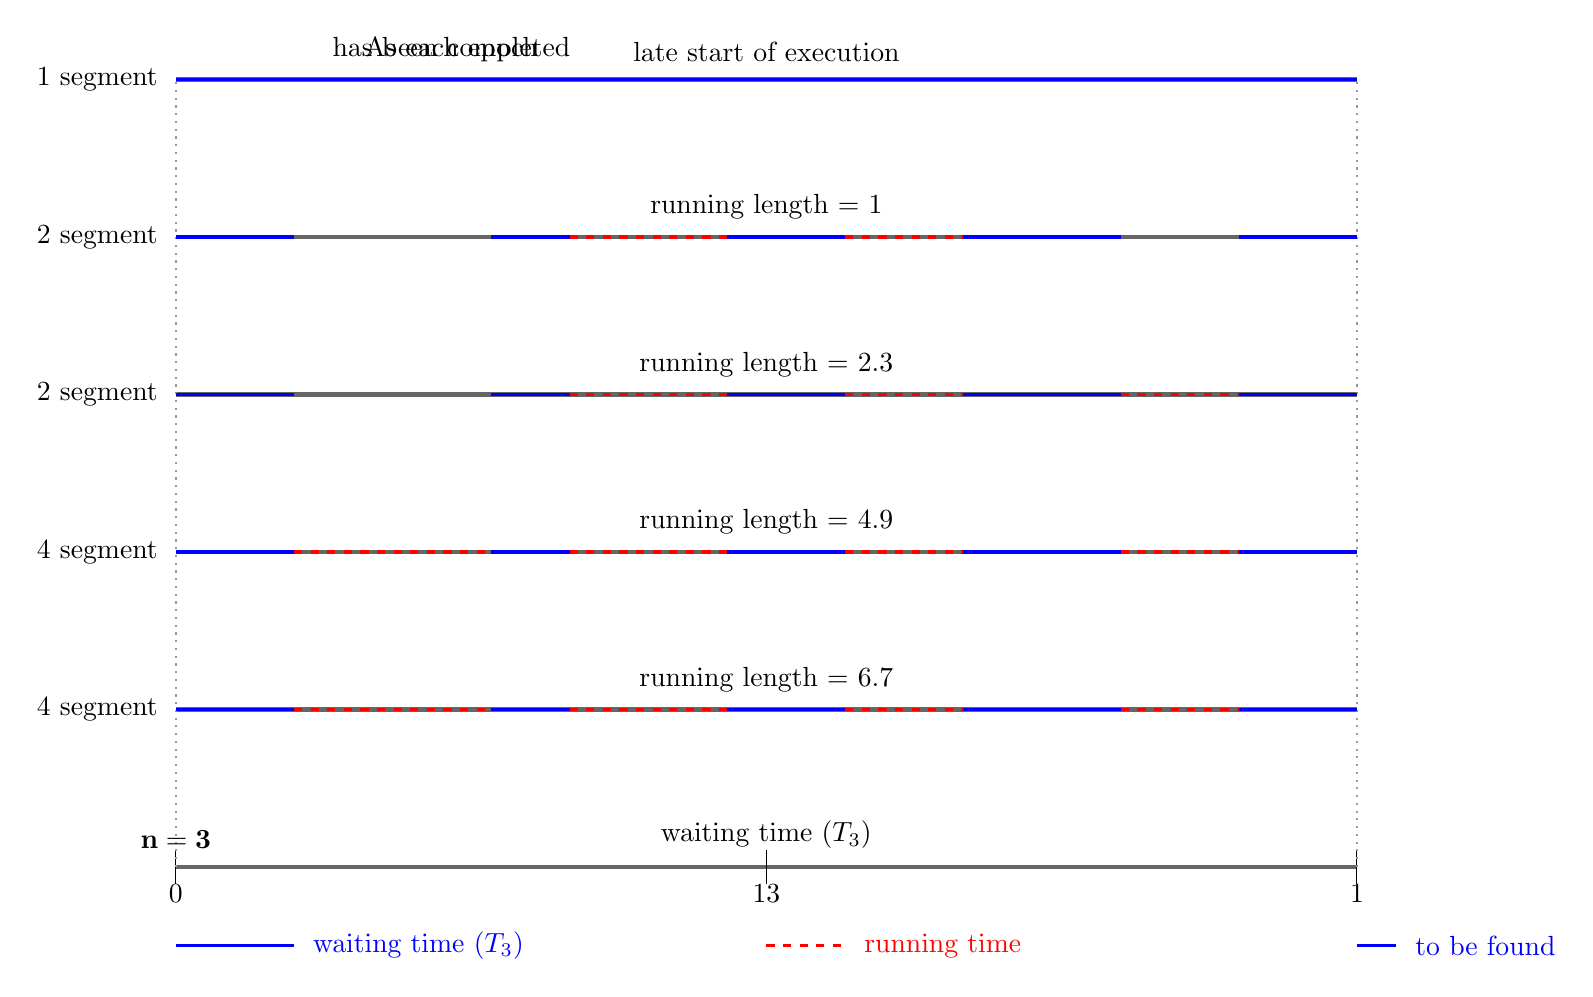
\begin{tikzpicture}
    % draw horizontal line   
    \draw[ultra thick,black!60] (0,0) -- (15,0);
    \draw[ultra thick,black!60] (0,2) -- (15,2);
    \draw[ultra thick,black!60] (0,4) -- (15,4);
    \draw[ultra thick,black!60] (0,6) -- (15,6);
    \draw[ultra thick,black!60] (0,8) -- (15,8);
    \draw[ultra thick,black!60] (0,10) -- (15,10);
    % draw vertical lines
    \foreach \x in {0,7.5,15}
    \draw (\x cm,6pt) -- (\x cm,-6pt);
    \draw[dotted, thick, black!40] (0,0) -- (0,10);
    \draw[dotted, thick, black!40] (15,0) -- (15,10);
    % draw node
    \draw (0,0) node[below=3pt] {$0$} node[above=3pt] {$\mathbf{n=3}$};
    \draw (7.5,0) node[below=3pt] {$13$} node[above=3pt] {waiting time $(T_{3})$};
    \draw (15,0) node[below=3pt] {$1$} node[above=3pt] {};
    \draw (0,2) node[left=3pt] {$4$ segment} node[above=3pt] {};
    \draw (0,4) node[left=3pt] {$4$ segment} node[above=3pt] {};
    \draw (0,6) node[left=3pt] {$2$ segment} node[above=3pt] {};
    \draw (0,8) node[left=3pt] {$2$ segment} node[above=3pt] {};
    \draw (0,10) node[left=3pt] {$1$ segment} node[above=3pt] {};
    \draw (7.5,2) node[above=3pt] {running length = $6.7$} node[above=3pt] {};
    \draw (7.5,4) node[above=3pt] {running length = $4.9$} node[above=3pt] {};
    \draw (7.5,6) node[above=3pt] {running length = $2.3$} node[above=3pt] {};
    \draw (7.5,8) node[above=3pt] {running length = $1$} node[above=3pt] {};
    \draw (7.5,10) node[above=3pt] {late start of execution} node[above=3pt] {};
    \draw (3.5,10) node[above=3pt] {As each epoch} node[above=3pt] {has been completed} node[above=3pt] {};
    \draw[red,dashed,very thick] (1.5,2) -- (4,2);
    \draw[red,dashed,very thick] (5,2) -- (7,2);
    \draw[red,dashed,very thick] (8.5,2) -- (10,2);
    \draw[red,dashed,very thick] (12,2) -- (13.5,2);
    \draw[red,dashed,very thick] (1.5,4) -- (4,4);
    \draw[red,dashed,very thick] (5,4) -- (7,4);
    \draw[red,dashed,very thick] (8.5,4) -- (10,4);
    \draw[red,dashed,very thick] (12,4) -- (13.5,4);
    \draw[red,dashed,very thick] (5,6) -- (7,6);
    \draw[red,dashed,very thick] (8.5,6) -- (10,6);
    \draw[red,dashed,very thick] (12,6) -- (13.5,6);
    \draw[red,dashed,very thick] (5,8) -- (7,8);
    \draw[red,dashed,very thick] (8.5,8) -- (10,8);
    \draw[blue,very thick] (0,2) -- (1.5,2);
    \draw[blue,very thick] (4,2) -- (5,2);
    \draw[blue,very thick] (7,2) -- (8.5,2);
    \draw[blue,very thick] (10,2) -- (12,2);
    \draw[blue,very thick] (13.5,2) -- (15,2);
    \draw[blue,very thick] (0,4) -- (1.5,4);
    \draw[blue,very thick] (4,4) -- (5,4);
    \draw[blue,very thick] (7,4) -- (8.5,4);
    \draw[blue,very thick] (10,4) -- (12,4);
    \draw[blue,very thick] (13.5,4) -- (15,4);
    \draw[blue,very thick] (0,6) -- (1.5,6);
    \draw[blue,very thick] (4,6) -- (5,6);
    \draw[blue,very thick] (7,6) -- (8.5,6);
    \draw[blue,very thick] (10,6) -- (12,6);
    \draw[blue,very thick] (13.5,6) -- (15,6);
    \draw[blue,very thick] (0,8) -- (1.5,8);
    \draw[blue,very thick] (4,8) -- (5,8);
    \draw[blue,very thick] (7,8) -- (8.5,8);
    \draw[blue,very thick] (10,8) -- (12,8);
    \draw[blue,very thick] (13.5,8) -- (15,8);
    \draw[blue,very thick] (0,10) -- (15,10);
    \draw[blue,very thick] (0,-1) -- (1.5,-1) node[right=3pt] {waiting time $(T_{3})$};
    \draw[red,dashed,very thick] (7.5,-1) -- (8.5,-1) node[right=3pt] {running time};
    \draw[blue,very thick] (15,-1) -- (15.5,-1) node[right=3pt] {to be found};
\end{tikzpicture}

\end{document}